\documentclass[11pt]{article}
%\usepackage{graphicx}
\usepackage{booktabs}
\usepackage[backend=bibtex]{biblatex}
%\addbibresource{myBibRefsFile.bib}
%\usepackage[backend=bibtex,style=verbose-trad2]{biblatex}
\bibliography{IT.bib}
\usepackage{float}

%\usepackage[margin=1in]{geometry}
\usepackage{fancyhdr}
%\pagestyle{fancy}
\usepackage{amsmath}
%\usepackage{amssymb}
%\usepackage[table]{xcolor}
\usepackage{bm}
\usepackage{array}
\usepackage{mathtools}
\usepackage{soul,soulutf8}
\usepackage{url,color}
\usepackage{fullpage}
\usepackage[english]{babel}

\usepackage[utf8]{inputenc}
\lhead{STA 4001: Stochastic Processes}
\chead{}
\rhead{\textup{CUHK(SZ) Fall 2018}}


\usepackage{amsmath,amsthm,amssymb}
%\usepackage{extarrows}
%\usepackage{breqn}
\usepackage{mathtools}
\DeclarePairedDelimiter\ceil{\lceil}{\rceil}
\DeclarePairedDelimiter\floor{\lfloor}{\rfloor}
\newcommand{\N}{\mathbb{N}}
\newcommand{\Z}{\mathbb{Z}}
\newcommand{\trans}{^{\mathrm T}}

\newenvironment{theorem}[2][Theorem]{\begin{trivlist}
\item[\hskip \labelsep {\bfseries #1}\hskip \labelsep {\bfseries #2.}]}{\end{trivlist}}
\newenvironment{lemma}[2][Lemma]{\begin{trivlist}
\item[\hskip \labelsep {\bfseries #1}\hskip \labelsep {\bfseries #2.}]}{\end{trivlist}}
\newenvironment{exercise}[2][Exercise]{\begin{trivlist}
\item[\hskip \labelsep {\bfseries #1}\hskip \labelsep {\bfseries #2.}]}{\end{trivlist}}
\newenvironment{reflection}[2][Reflection]{\begin{trivlist}
\item[\hskip \labelsep {\bfseries #1}\hskip \labelsep {\bfseries #2.}]}{\end{trivlist}}
\newenvironment{proposition}[2][Proposition]{\begin{trivlist}
\item[\hskip \labelsep {\bfseries #1}\hskip \labelsep {\bfseries #2.}]}{\end{trivlist}}
\newenvironment{corollary}[2][Corollary]{\begin{trivlist}
\item[\hskip \labelsep {\bfseries #1}\hskip \labelsep {\bfseries #2.}]}{\end{trivlist}}
\DeclareMathOperator{\tr}{tr}
\DeclareMathOperator{\rank}{rank}
\DeclareMathOperator{\Span}{span}
\DeclareMathOperator{\row}{row}
\DeclareMathOperator{\col}{col}
\DeclareMathOperator{\range}{range}
\DeclareMathOperator{\Null}{Null}
\DeclarePairedDelimiterX{\inp}[2]{\langle}{\rangle}{#1, #2}
\DeclareMathOperator{\Proj}{Proj}
\newcommand{\diff}{\,\mathrm{d}}
\DeclareMathOperator{\trace}{trace}
\newcommand{\Her}{^{\mathrm H}}
\DeclareMathOperator{\diag}{diag}
\newcommand{\Var}{\mathrm{Var}}
%\usepackage{listings}
%\usepackage{color} %red, green, blue, yellow, cyan, magenta, black, white
%\definecolor{mygreen}{RGB}{28,172,0} % color values Red, Green, Blue
%\definecolor{mylilas}{RGB}{170,55,241}
%
%
%\lstset{language=Matlab,%
%    %basicstyle=\color{red},
%    breaklines=true,%
%    morekeywords={matlab2tikz},
%    keywordstyle=\color{blue},%
%    morekeywords=[2]{1}, keywordstyle=[2]{\color{black}},
%    identifierstyle=\color{black},%
%    stringstyle=\color{mylilas},
%    commentstyle=\color{mygreen},%
%    showstringspaces=false,%without this there will be a symbol in the places where there is a space
%    numbers=left,%
%    numberstyle={\tiny \color{black}},% size of the numbers
%    numbersep=9pt, % this defines how far the numbers are from the text
%    emph=[1]{for,end,break},emphstyle=[1]\color{red}, %some words to emphasise
%    %emph=[2]{word1,word2}, emphstyle=[2]{style},    
%}
\usepackage{listings}
\RequirePackage{listings}
\RequirePackage{xcolor}
\definecolor{dkgreen}{rgb}{0,0.6,0}
\definecolor{gray}{rgb}{0.5,0.5,0.5}
\definecolor{mauve}{rgb}{0.58,0,0.82}
\lstset{
  frame=tb,
  aboveskip=3mm,
  belowskip=3mm,
  showstringspaces=false,
  columns=flexible,
  framerule=1pt,
  rulecolor=\color{gray!35},
  backgroundcolor=\color{gray!5},
  basicstyle={\small\ttfamily},
  numbers=none,
  numberstyle=\tiny\color{gray},
  keywordstyle=\color{blue},
  commentstyle=\color{dkgreen},
  stringstyle=\color{mauve},
  breaklines=true,
  breakatwhitespace=true,
  tabsize=3,
}

\newcommand{\degree}{\ensuremath{^\circ}}
\begin{document}
\title{\bfseries\upshape{Solution to Assignment 2}}%replace X with the appropriate number
\author{\textit{I will appreciate it if you could give me some advice on my assignment!}} %if necessary, replace with your course title
\maketitle
\begin{enumerate}
\item
Let $f$ be \emph{twice continuously differentiable}. Suppose that $x^*$ is a local minimum such that for all $x$ in an open sphere $S$ centered at $x^*$, we have, for some $m>0$,
\[
\begin{array}{ll}
m\|d\|^2\le d'\nabla^2 f(x)d,
&
\forall d\in\mathbb{R}^n
\end{array}
\]
Show that for every $x\in S$, we have 
\[
\|x-x^*\|\le\frac{\|\nabla f(x)\|}{m},
\qquad
\|f(x) - f(x^*)\|\le\frac{\|\nabla f(x)\|^2}{2m}
\]
\begin{proof}
The idea for the estimation of $\|x-x^*\|$ is to build the estimation of $\nabla f(x)-\nabla f(x^*)$:
\begin{subequations}
\begin{align}
\nabla f(x)&=\nabla f(x^*)+\int_0^1\nabla^2f(x^*+t(x-x^*))(x-x^*)\diff t\\
&=\int_0^1\nabla^2f(x^*+t(x-x^*))(x-x^*)\diff t
\end{align}
Leftmultiplying $(x-x^*)'$ both sides, we obtain:
\begin{align}
\inp{\nabla f(x)}{(x-x^*)}&=(x-x^*)'*\int_0^1\nabla^2f(x^*+t(x-x^*))(x-x^*)\diff t\\
&=\int_0^1(x-x^*)'\nabla^2f(x^*+t(x-x^*))(x-x^*)\diff t\\
&\ge \int_0^1m\|x-x^*\|^2\diff t=m\|x-x^*\|^2
\end{align}
By applying Cauchy-Schwarz inequality for LHS, we derive:
\[
\|\nabla f(x)\|\cdot\|x-x^*\|\ge \inp{\nabla f(x)}{(x-x^*)}\ge m\|x-x^*\|^2,
\]
by re-arranging terms we imply $\|x-x^*\|\le\frac{\|\nabla f(x)\|}{m}$.
\end{subequations}

The estimation of $\|f(x) - f(x^*)\|$ relies on the taylor expansion:
\begin{subequations}
Expanding $f(x^*)$ into 2nd order, we obtain:
\begin{equation}
f(x^*) = f(x) + \inp{\nabla f(x)}{(x^* - x)} + \frac{1}{2}(x^*-x)'\nabla^2f(z)(x^*-x),
\end{equation}
for some $z$ between $x^*$ and $x$. Since $z$ is still in the sphere $S$, we obtain:
\begin{equation}
f(x^*) - f(x) \ge\inp{\nabla f(x)}{(x^* - x)} +  \frac{m}{2}\|x^*-x\|^2
\end{equation}
Note that the RHS has a lower bound:
\begin{equation}\label{Eq:2:c}
\inp{\nabla f(x)}{(x^* - x)} +  \frac{m}{2}\|x^*-x\|^2
\ge
\min_{y}\inp{\nabla f(x)}{(y - x)} +  \frac{m}{2}\|y-x\|^2
\end{equation}
Solving the quadratic minimization, i.e., taking the derivative w.r.t. $y$ leads to $m(y-x)+\nabla f(x)=0\implies y^* = x-\frac{\nabla f(x)}{m}$ and
\begin{equation}\label{Eq:2:d}
\min_{y}\inp{\nabla f(x)}{(y - x)} +  \frac{m}{2}\|y-x\|^2
=
-\frac{1}{2m}\|\nabla f(x)\|^2
\end{equation}
Substituting $(\ref{Eq:2:d})$ into (\ref{Eq:2:c}), we derive:
\begin{align*}
f(x^*) - f(x) &\ge\inp{\nabla f(x)}{(x^* - x)} +  \frac{m}{2}\|x^*-x\|^2\\
&\ge -\frac{1}{2m}\|\nabla f(x)\|^2
\end{align*}
Or equivalently,
\begin{equation}
\|f(x^*) - f(x)\|=f(x) - f(x^*)\le \frac{1}{2m}\|\nabla f(x)\|^2
\end{equation}
since $f(x^*)=\inf_{x}f(x)$.
\end{subequations}






\end{proof}
\item
Suppose that a vector sequence $\{\bm e^k\}$ satisfies
\[
\begin{array}{ll}
\|\bm e^{k+1} - \bm e^k\|\le\beta\|\bm e^k - \bm e^{k-1}\|,
&
\forall k\ge \bar k
\end{array}
\]
wher e$\bar k$ is a positive integer and $\beta\in(0,1)$ i s a scalar. Show that $\{\bm e^k\}$ converges to some vector $\bm e^*$ linearly, and in fact we have
\[
\|\bm e^k - \bm e^*\|\le q\beta^k
\]
for some scalar $q$ and all $k$.
\begin{proof}
\begin{itemize}
\item
Firstly we show that $\{\bm e^k\}$ is Cauchy. For $\forall k\ge \bar k$, we have:
\[
\|\bm e^{k+1} - \bm e^k\|\le\beta\|\bm e^k - \bm e^{k-1}\|
\le\beta^2\|\bm e^{k-1} - \bm e^{k-2}\|\le\cdots\le
\beta^{k+1-\bar k}\|\bm e^{\bar k} - \bm e^{\bar k-1}\|
\]
Hence, for $\forall m,n\ge N\ge \bar k$, we have: (suppose $m\ge n$ w.l.o.g.)
\begin{align*}
\|\bm e^m -\bm e^n\|&\le \|\bm e^{m} - \bm e^{m-1}\|+\cdots
+
\|\bm e^{n+1} - \bm e^n\|\\
&\le \left(\beta^{m - \bar k}+\beta^{m-1-\bar k}+\cdots+\beta^{n+1-\bar k}\right)\|\bm e^{\bar k} - \bm e^{\bar k - 1}\|\\
&=\beta^{-\bar k}\|\bm e^{\bar k} - \bm e^{\bar k - 1}\|\sum_{i=n+1}^{m}\beta^i
\end{align*}
As $N$ goes sufficently large, we can make the partial series $\sum_{i=n+1}^{m}\beta^i$ arbitrarily small. Therefore, $\|\bm e^m-\bm e^n\|\to0$ as $N\to\infty$, hence $\{\bm e^k\}$ is Cauchy.
\item
For any $m\ge k\ge \bar k$, by applying the same trick,
\begin{equation}\label{Eq:3}
\|\bm e^m - \bm e^k\|\le 
\beta^{-\bar k}\|\bm e^{\bar k} - \bm e^{\bar k - 1}\|\sum_{i=k+1}^{m}\beta^i
\end{equation}
Since $\{\bm e^k\}$ is Cauchy, it has a limit, say, $\lim_{k\to\infty}\bm e^k=\bm e^*$. Taking limit both sides for (\ref{Eq:3}) as $m\to\infty$, we obtain that for $\forall k\ge\bar k$,
\begin{equation}\label{Eq:4}
\|\bm e^k - \bm e^*\|\le 
\beta^{-\bar k}\|\bm e^{\bar k} - \bm e^{\bar k - 1}\|\sum_{i=k+1}^{\infty}\beta^i
=\beta^{-\bar k}\|\bm e^{\bar k} - \bm e^{\bar k - 1}\|
\frac{\beta^{k+1}}{1-\beta}
:=M\beta^k
\end{equation}
with $M=\frac{\beta^{-\bar k+1}}{1-\beta}\|\bm e^{\bar k} - \bm e^{\bar k - 1}\|$.

We define $M_1:=\max_{1\le k<\bar k}\frac{\|\bm e^k-\bm e^*\|}{\beta^k}$, immediately we obtain:
\begin{equation}\label{Eq:5}
\begin{array}{ll}
\|\bm e^k-\bm e^*\|\le M_1\beta^k,
&
1\le k<\bar k
\end{array}
\end{equation}
Combining (\ref{Eq:4}) and (\ref{Eq:5}), we imply for any $k$, the inequality holds:
\[
\|\bm e^k-\bm e^*\|\le q\beta^k,
\]
where $q:=\max\{M,M_1\}$.
\end{itemize}



\end{proof}













\end{enumerate}

\clearpage
\section*{MATLAB Code Copy}
\subsection*{Code Copy for LP}
\begin{lstlisting}[language=matlab]
function x = myL1reg0(A, b, D)
% This function solves the optimizatin problem
% Input:
%       A: a m*n matrix
%       b: a m*1 vector
%       D: a k*n matrix
% minimize sum_{i=1}^m t_i
% such that A * x = b
% for i = 1:k,
%        - t_i \le \sum_{j=1}^n d_{ij}x_j \le t_i
% construct decision variable X = [x_1,...,x_n,s_1,...,s_m]';
%% Estimate size
[m,n] = size(A);
[k,~] = size(D);

%% Construct f, Aineq, bineq, Aeq, beq
f(n+1:n+k) = 1;
Aineq = [D,-1 * eye(k); -1 *D, -1 * eye(k)];
bineq = zeros(k+k,1);
Aeq = [A,zeros(m,k)];
beq = b;
%% Use Linprog to solve optimization
options = optimoptions('linprog','Algorithm','interior-point','MaxIter',20,...
    'OptimalityTolerance',5e-4,'ConstraintTolerance',1e-4,'Display','off');
X = linprog(f,Aineq,bineq,Aeq,beq,[],[],options);

x = X(1:n);

end 
\end{lstlisting}
\subsection*{Code Copy for SD}
\begin{lstlisting}[language=matlab]
function [x,iter] = myL1reg1(A, b, D)
% Input: 
%     A: a m*n matrix
%     b: a m*1 vector
%     D: a k*n matrix
% Usage:
%     solve the unconstrained minimization model
%     min phi_sigma(D * x) + mu/2 * ||A*x - b||_2^2
% with
% sigma = 0.05 around
% mu = 0.1 around
% phi_sigma(y) = \sum_{i=1}^k(y_i^2+sigma)^(1/2)

%% parameters setting
sigma = 5e-2;   mu = 1e-1;
object = @(x,Dx) sum(sqrt(((Dx).^2+sigma))) + mu/2 * norm(A*x - b)^2;
nabla = @(x,Dx) ((Dx./sqrt(Dx.^2 + sigma))'*D)'+(mu*(A*x - b)' * A)';
tol_2 = 1e-7;
maxiter = 50000;    
beta = 0.5;   
C1 = 1e-5;
%% initial setting
x = A' * ((A*A')\b); 
Dx = D*x;
f = object(x,Dx);   
g = nabla(x,Dx);   
gnorm = norm(g);    %gnorm0 = gnorm
tol_1 = gnorm * 5e-2;
alpha = 1;  %initial step-size

%% Iteration Running
for iter = 1:maxiter
    delta = C1 * alpha * gnorm^2;
    Dg = D*g;
    for arm = 1:10
        % Armijo Condition
        x_try = x - alpha * g;
        Dx_try = Dx - alpha * Dg;
        f_try = object(x_try,Dx_try);
        if f_try <= f - delta,break; end
        alpha = alpha * beta;
    end
    % update function
    x_pre = x;  g_pre = g;    f_diff = 1 - f_try/f;
    x = x_try;  Dx = Dx_try;  g = nabla(x,Dx); 
    f = f_try;  gnorm = norm(g);
    if gnorm <= tol_1   && f_diff <= tol_2, break; end
    % BB step
    s = x - x_pre;  y = g - g_pre;
    alpha = (s'*y) / (y' * y);
end
end
\end{lstlisting}

\clearpage
\section*{Matlab screen printout of LP Run}
\begin{figure}[H]
\centering
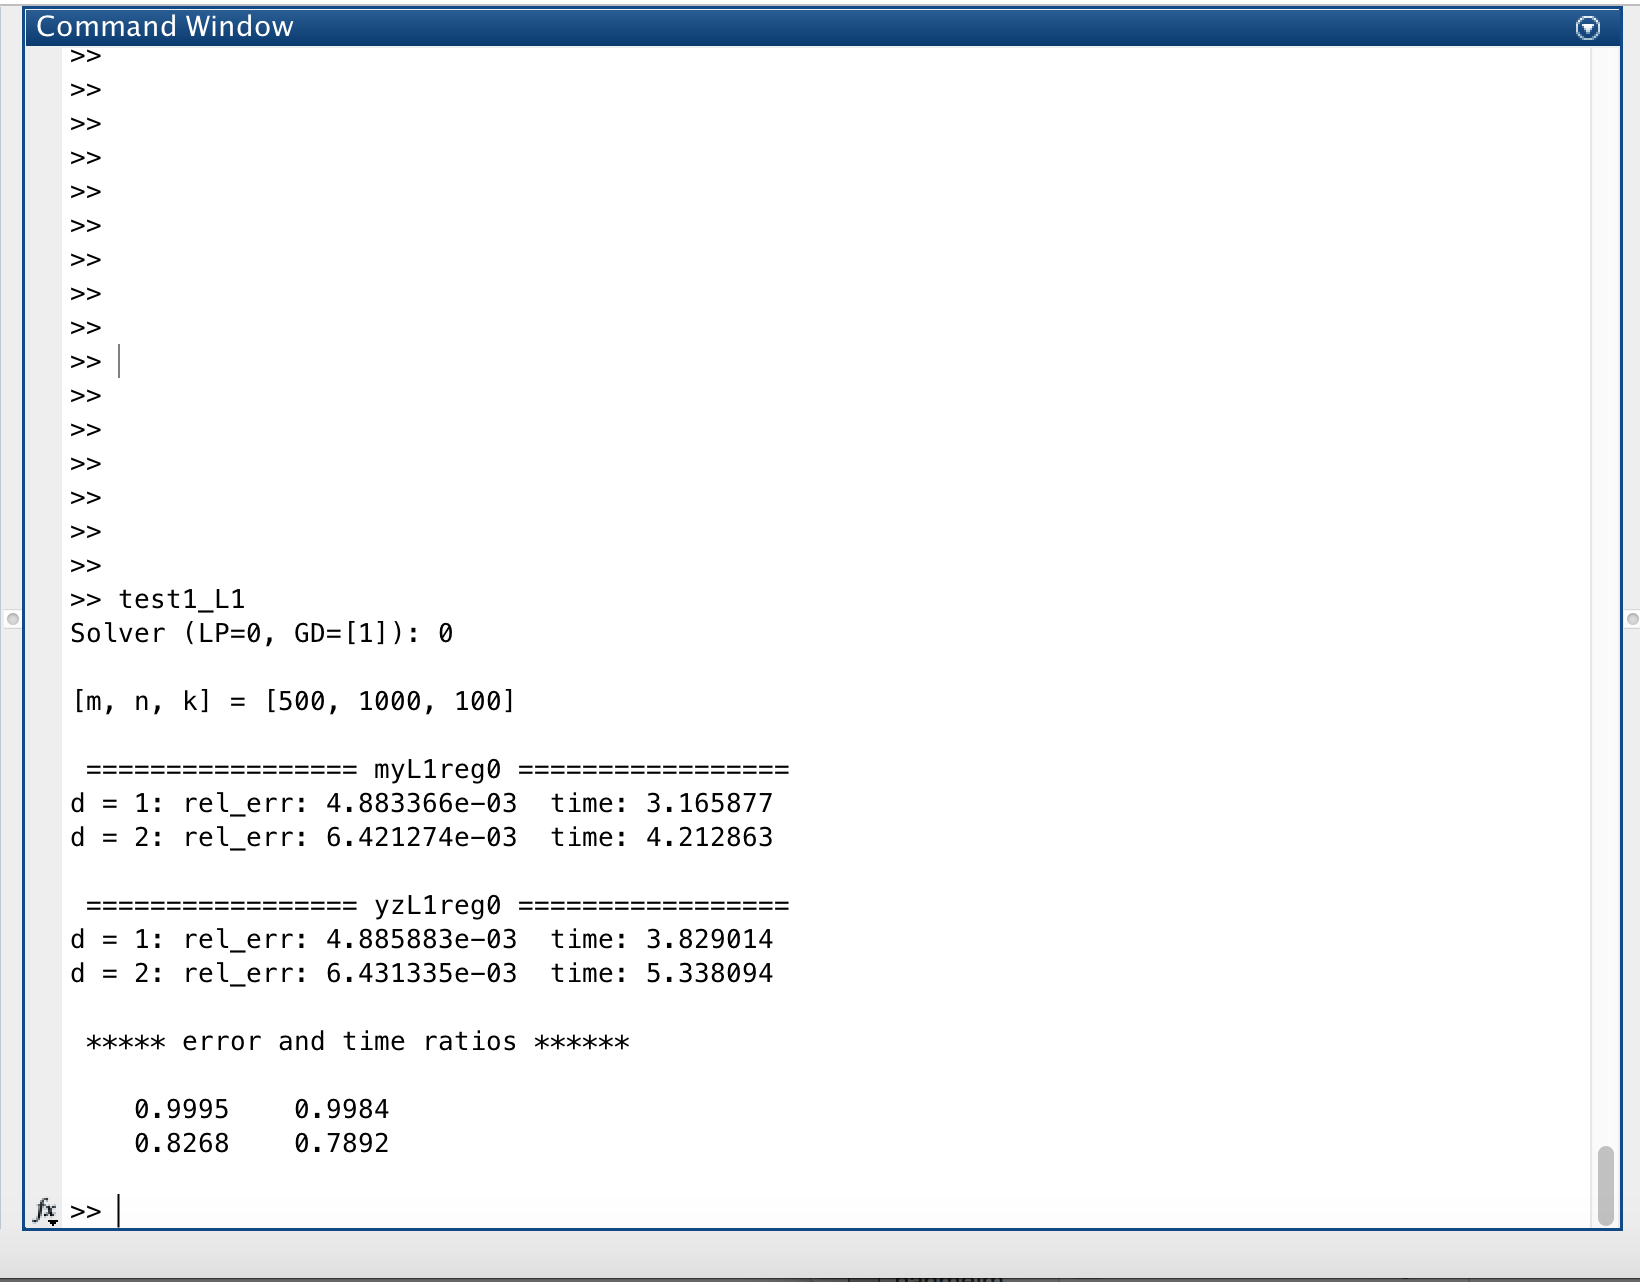
\includegraphics[height=12cm]{LP}
\caption{Printout from Run (LP)}
\label{Printout from Run}
\end{figure}

\clearpage
\section*{Matlab screen printout of SD Run}
\begin{figure}[H]
\centering
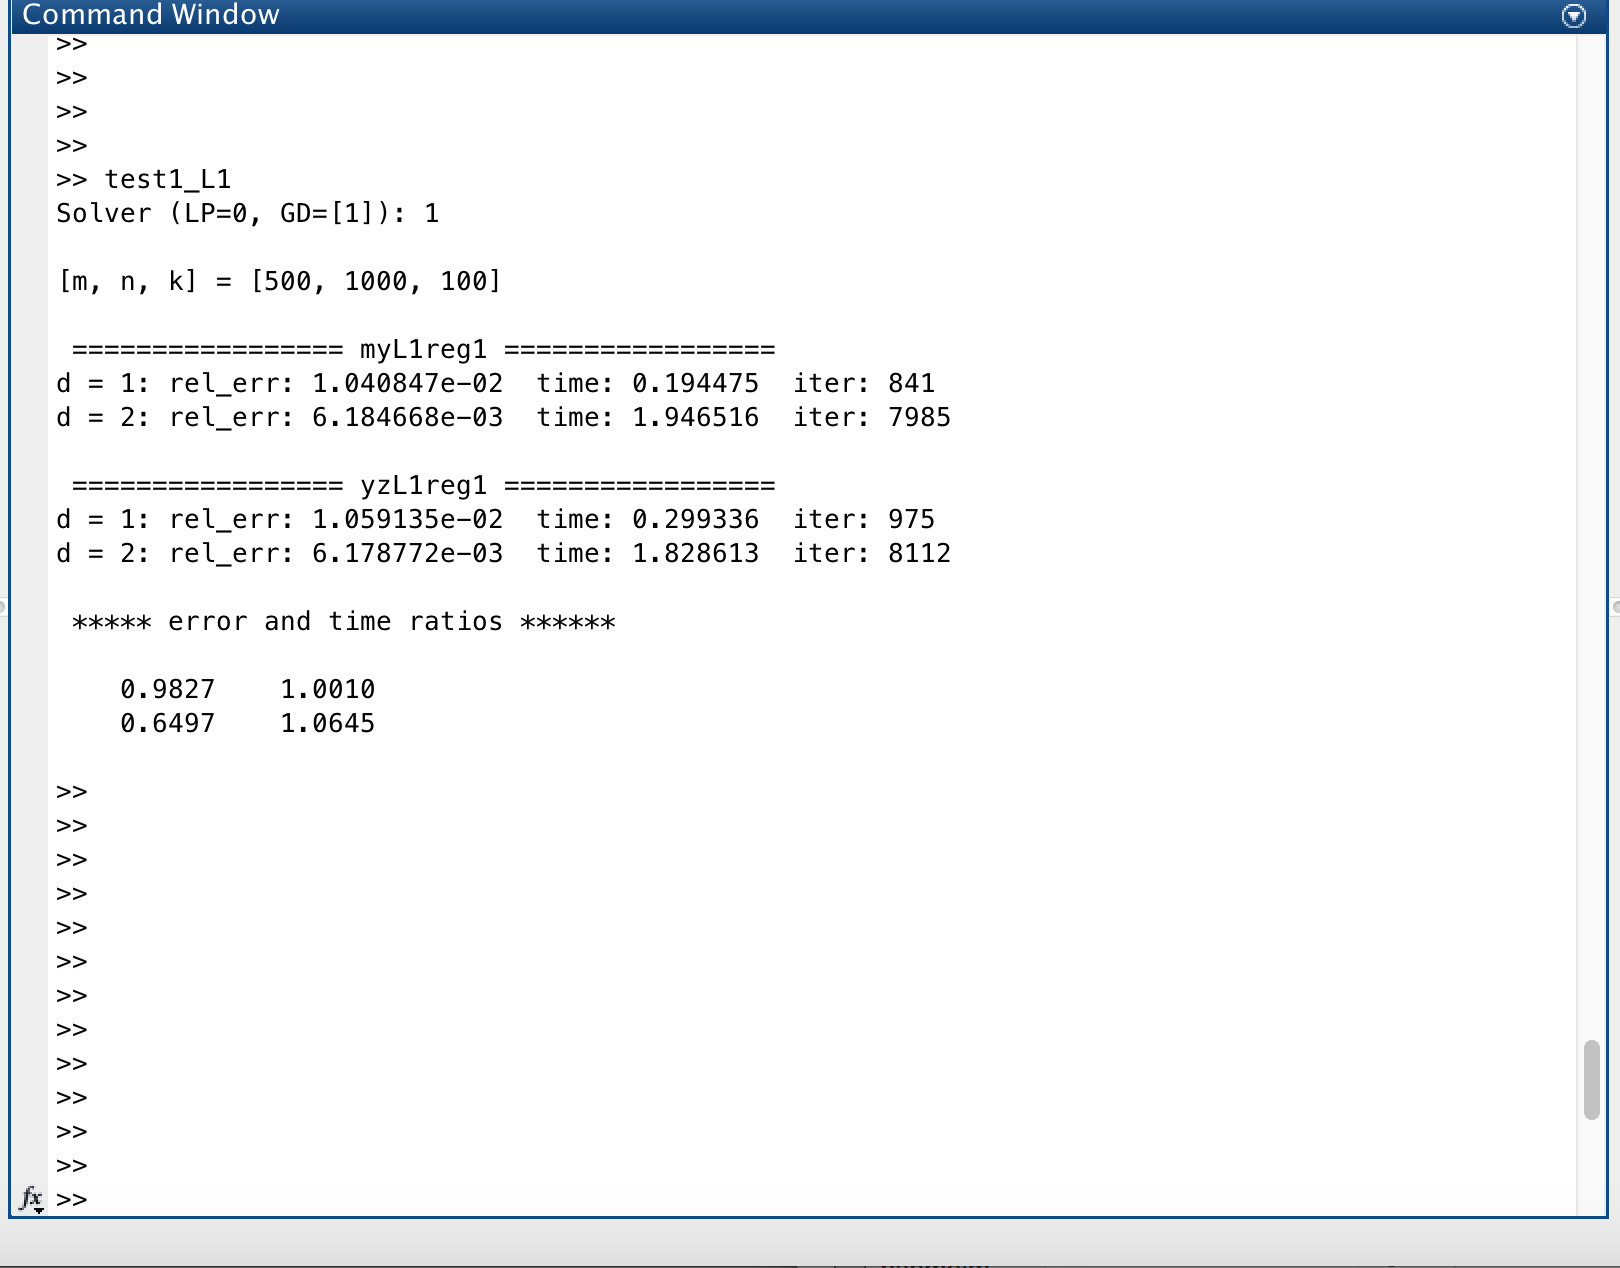
\includegraphics[height=12cm]{SD}
\caption{Printout from Run (SD)}
\end{figure}

\clearpage
\section*{Output figures from LP solvers}
\begin{figure}[H]
\centering
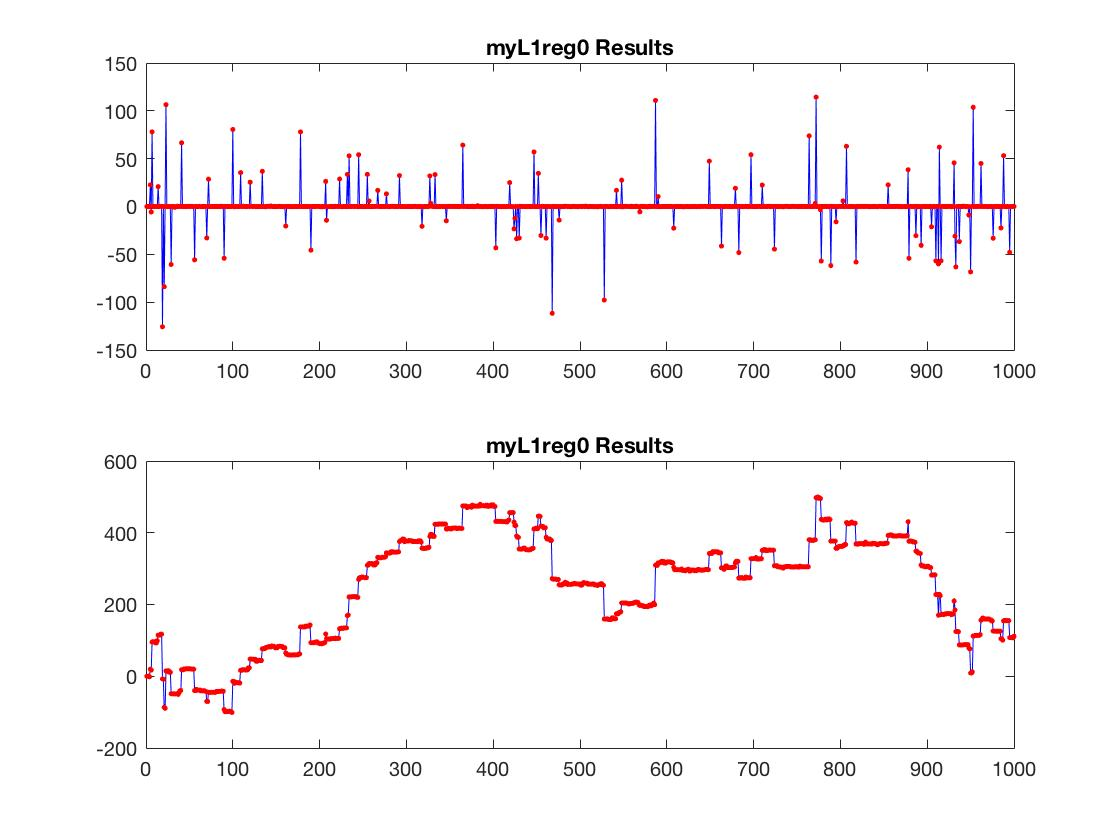
\includegraphics[height=10cm]{Output_1}
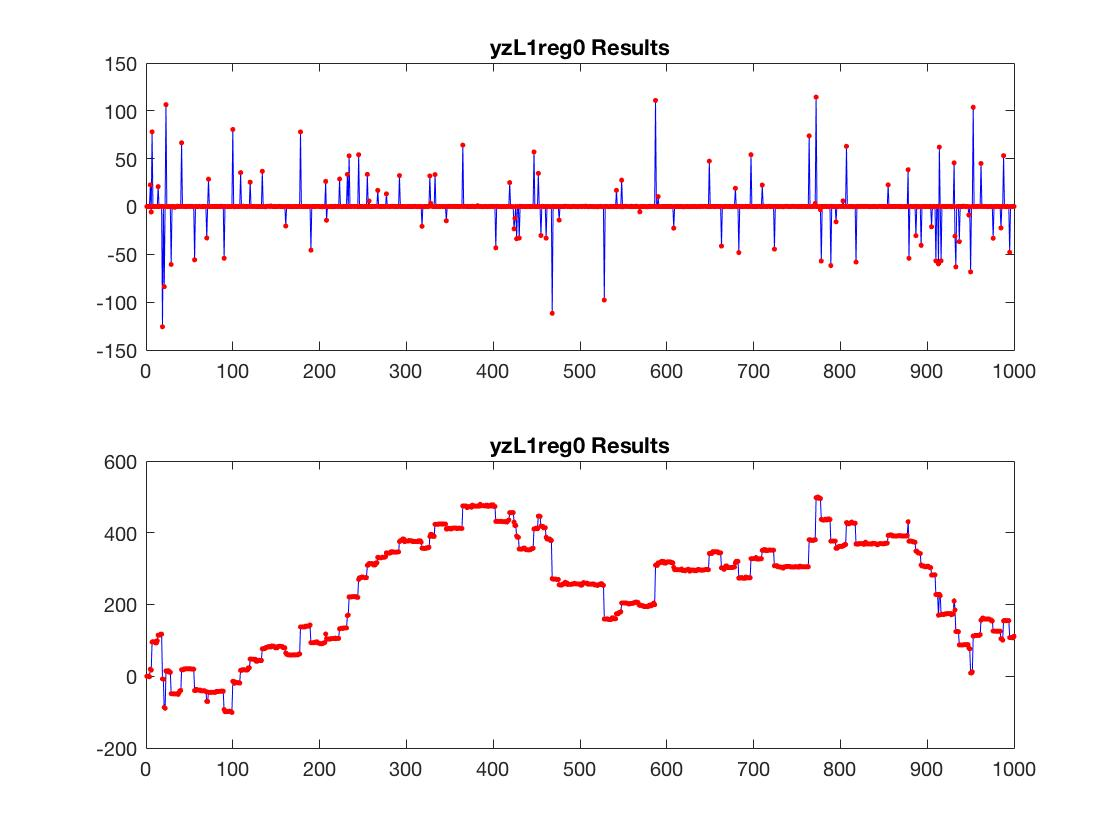
\includegraphics[height=10cm]{Output_2}
\caption{Output figures from LP solvers}
\end{figure}
\clearpage
\section*{Output figures from SD solvers}
\begin{figure}[H]
\centering
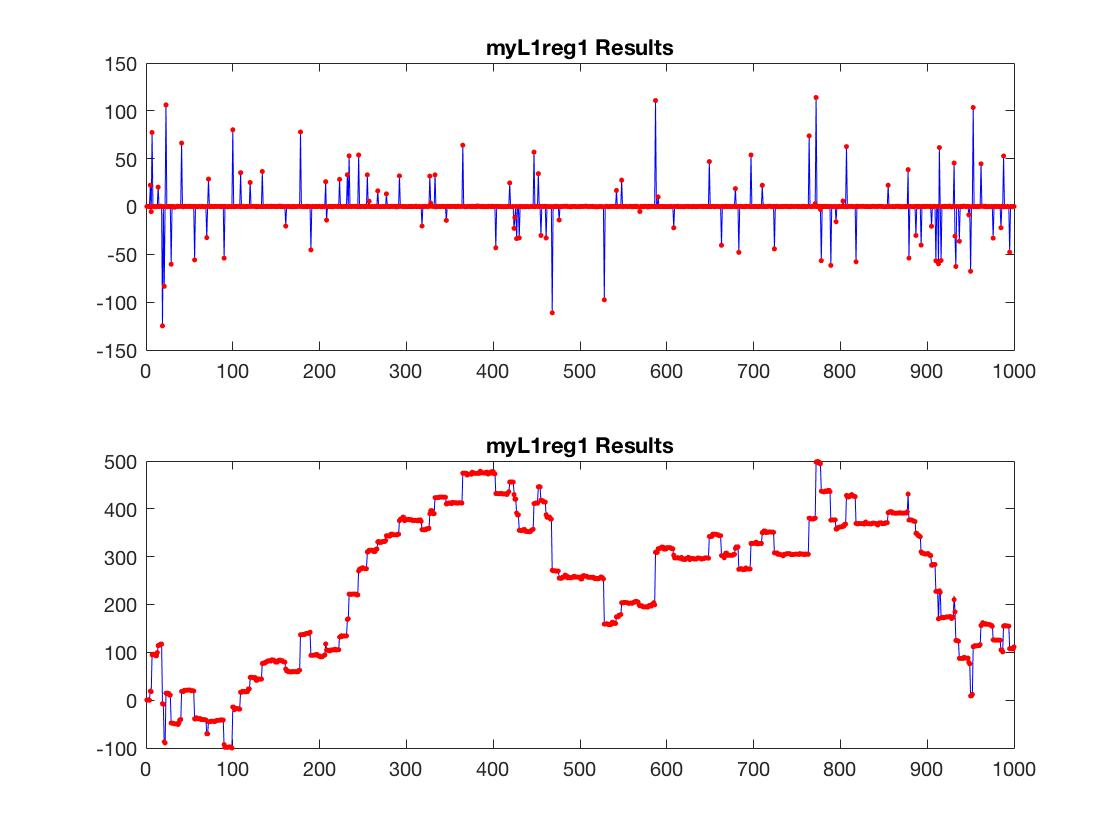
\includegraphics[height=10cm]{Output_4}
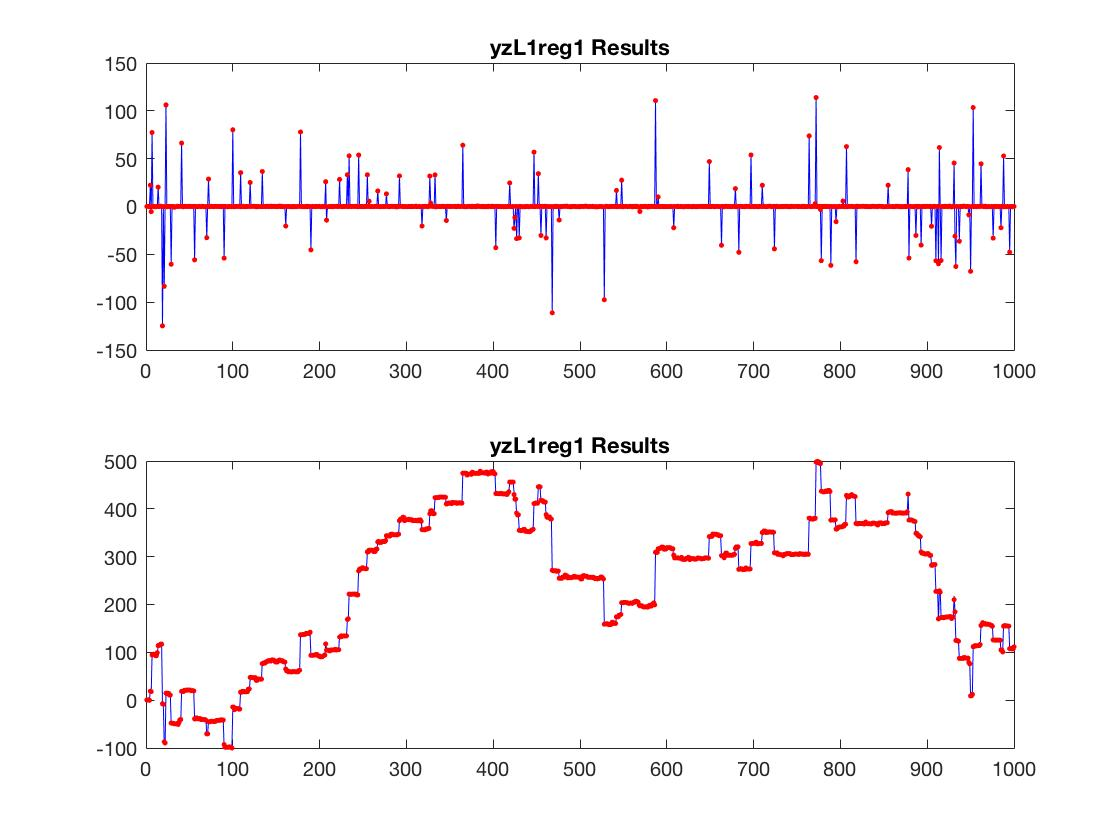
\includegraphics[height=10cm]{Output_3}
\caption{Output figures from SD solvers}
\end{figure}

\clearpage
\section*{A short summary}
\paragraph{Introduction}
This project is to recover a desired signal by L1 Regularization method. Firstly we consider a linear programming approach; then we consider an unconstrained minimization model, which can be solved by steepest gredient descent.

\paragraph{Practice Requirement}
The LP approach cannot meet the optimal solution in practice in general as the constraint requires the \emph{exact} solution to the under-determined linear system $\bm{Ax}=\bm b$. However, in practice there are always some errors between $\bm{Ax}=\bm b$ due to the noise. Alternatively, the SD model can handle such case well via adding the penalty term $\|\bm{Ax}-\bm b\|_2^2$. This penalty term gives us the approximate solution to the linear system.
\paragraph{Running Time}
The running time for LP approach is generally slower than that for SD approach. That's because for this large-scale optimization problem, the LP solver has to handle large size matrices (necessarily not be sparse), which is not efficient. In constrast, the SD solver only need to compute operations on vectors (gredient) per iteration, which is efficient.
\paragraph{Choice of Step-size}
However, the disadvantage of SD approach is that the choice of step-size is a kind of art. There is no principal way that can recommend the step-size for all or even most problems. Careful analysis on the optimization problem is necessary. A bad example is that if we disable BB steps and always initialize $\alpha=1$ in the back tracking, the running time is sensitive to the scale of optimization problem. Look at the screen printout of this runs:
\begin{figure}[H]
\centering
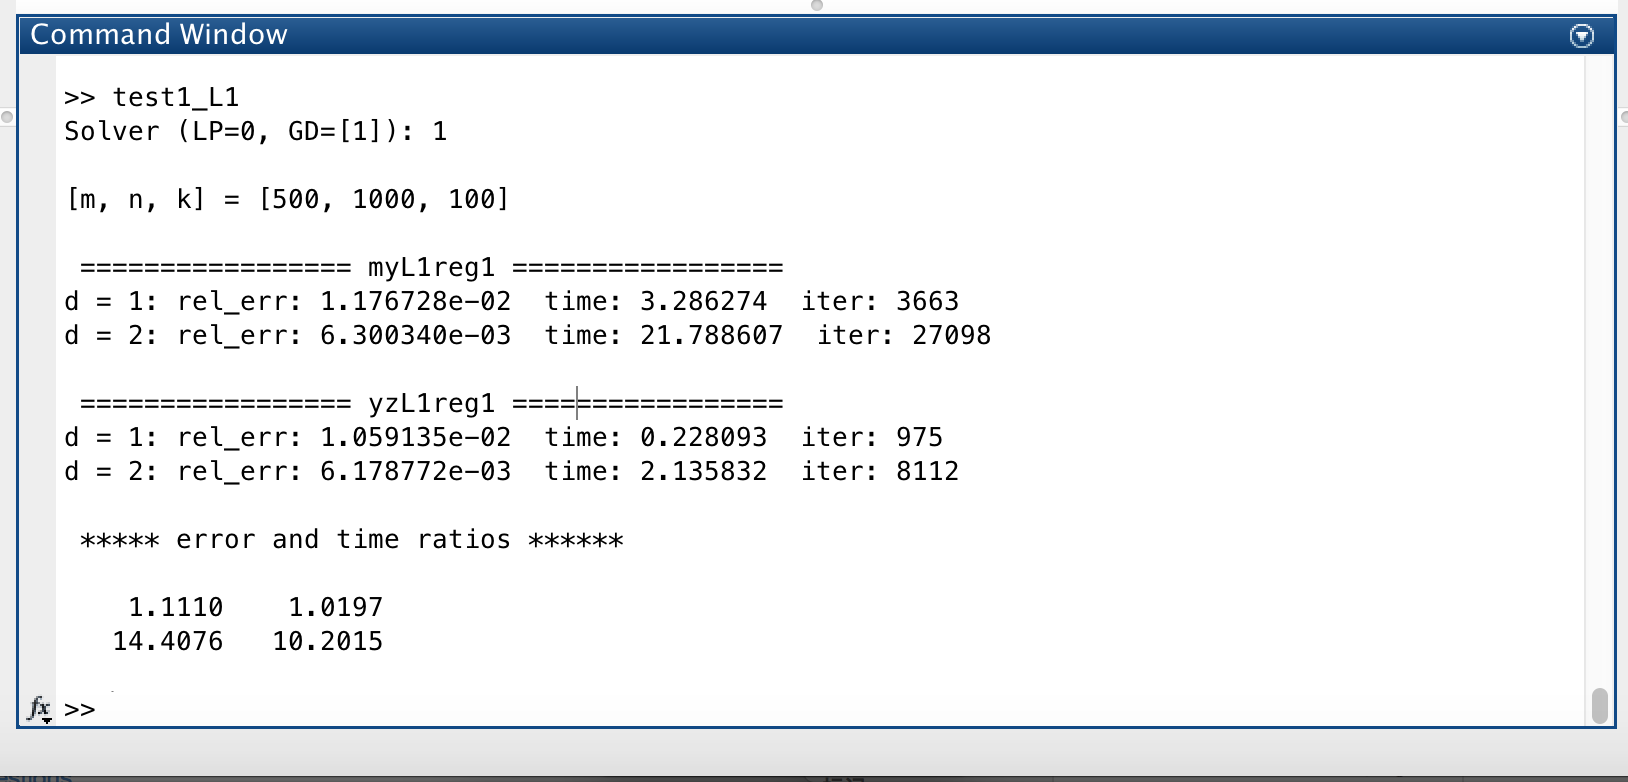
\includegraphics[width=10cm]{Test}
\caption{screen printout of disabled-BB-step results}
\end{figure}
\paragraph{Efficient LP Approach}
The advantage of LP appraoch is that there is indeed a muture way to solve this problem in polynomial time. The interior point method is one of the best way to solve the large-scale LP problem.











\end{document}